\chapter{Experiments}
\label{ch:experiments}

\section{Datasets}
\label{sec:ds}

In this section we consider datasets that are separated in two opposing communities. The information about the opinions of each member of this community is known. Thus, we can assign internal opinions -1 and 1 to the nodes depending on their community membership\cite{tsapMatakosTerzi}.  We consider the following.

\begin{enumerate}

  \item The Karate dataset, that represents the friendships between the members of a karate club at a US university. This network is split in two equal size polarized communities around two rival karate instructors.
  
  \item The Books dataset, that is a network of US politics books. These books were published near the 2004 presidential election and sold by Amazon. These Books are classified as "Liberal", "Conservative", or "Neutral".  There are in total 43 liberal books, 49 conservative and 13 neutral.
  
  \item The Blogs dataset, a network of hyperlinks between online blogs on US politics. Blogs are classified as either Liberal or Conservative.
  
  \item The Elections dataset, this dataset is the network between the Twitter followers of Hillary Clinton and Donald Trump collected in the period 15/12/2016-15/01/2017 – around the time of the 2016 presidential elections. Members of this network are assigned an internal opinion of 1 or -1 based on which one of the two candidates they follow. We took a subsampled portion that has be created by Matakos, et al \cite{tsapMatakosTerzi}.
    
  \item The beefban dataset, a  hashtag that Twitter users used in March 2015 to signal that their posts referred to a decision by the Indian government about the consumption of beef meat in India.
  
  \item The GermanWings dataset, a  hashtag that Twitter users used after the crash of GermanWings Flight 9525.
  
\end{enumerate}

\vspace{23pt}

We present some statistics for the datasets in the Table \ref{tab:statistics}.
\vspace{36pt}

\begin{table}[H]
 \centering
 \caption{Statistics}
 \label{tab:statistics}
 \begin{tabular}{| l || l | l | l | l |}
 \hline
  Name & \# of Nodes & \# of Edges & Avg. Degree & $\pi(z)$\\
  \hline
  \hline
  Karate & $34$ & $78$ & 4.5882 &  0.33964\\
  \hline
    books & $105$ & $441$ & 8.4 &  0.43429\\
  \hline
    beefban & $799$ & $6026$ & 15.0839 &  0.30326\\
  \hline
  polblogs & $1490$ & $16718$ & 22.4403 &  0.30983\\
  \hline
  GermanWings & $2111$ & $7329$ & 6.9436 &  0.44479\\
  \hline
  ClintonTrump & $2832$ & $18551$ & 13.1010 &  0.07582\\
  \hline
 \end{tabular}
 \end{table}
 
\clearpage

\section{Experiments}
\label{sec:experim}

We now present experiments with our algorithms for the $k-Addition$ problem. In addition to the heuristics we use two random algorithms. The $Random$, that chooses random edges from all possible combinations and the $RandomDifferent$. The second one chooses random edges between different $z$ opinions. More specifically edges that the multiplication of their expressed opinions is negative ($z_u*z_v < 0$). 
\\
\\
We can experiment with all algorithms only for the $Karate$ and the $Books$ datasets. The $Greedy$ algorithm, that recomputes $\pi(z)$ for every candidate edge cannot run on the rest of the datasets that contain thousands of nodes.The $FirstTopGreedy$ and the $Expressed Opinion$ run in all datasets.
\\
\\
In figure~\ref{fig:heuristics_small} we plot the decrease of the polarization index of the heuristics for all our algorithms. We make the following observations.
\clearpage

\begin{figure}[!htbp]
	\begin{center}
	\advance\leftskip-1.3cm
	\captionsetup{justification=centering,margin=2cm}
	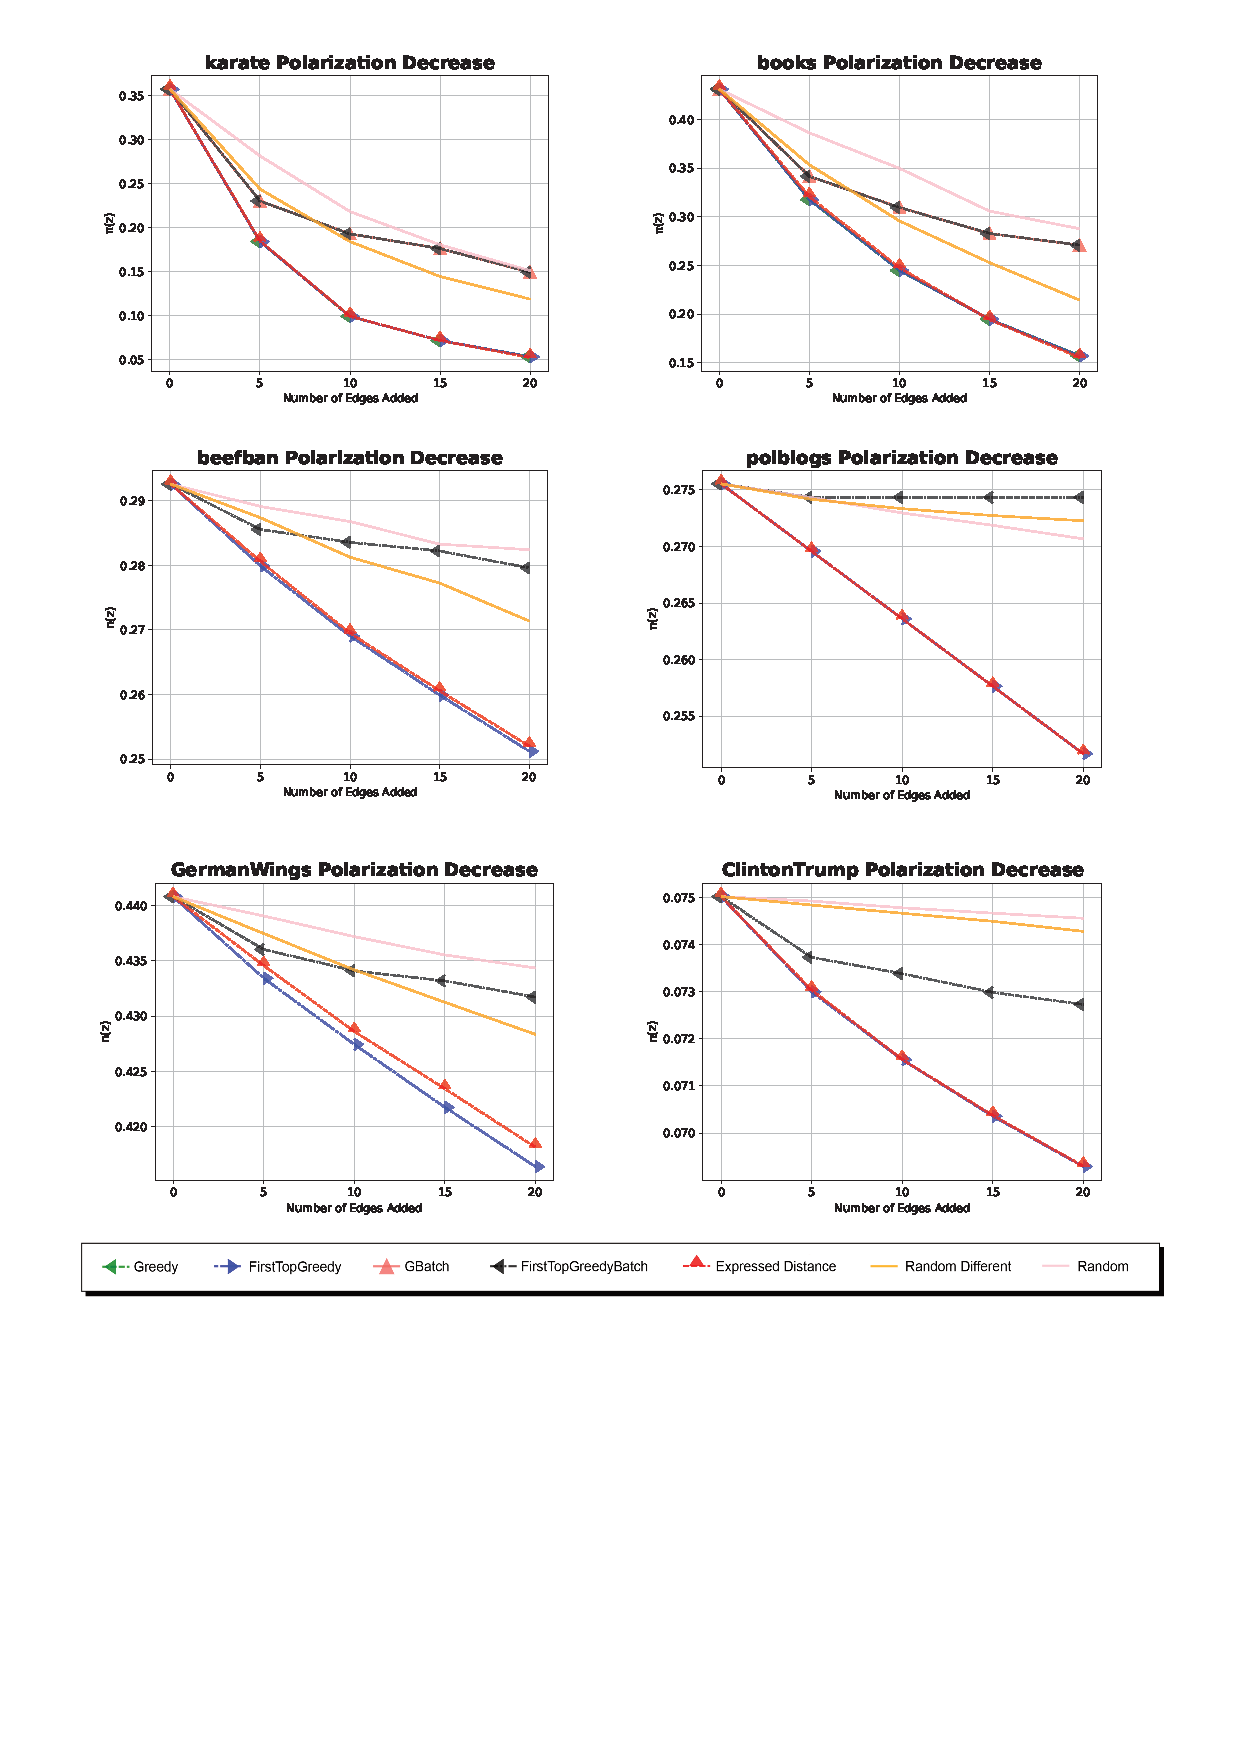
\includegraphics[width=1.2\textwidth]{Figures/heuristics}
	\caption{Comparison of the heuristics between datasets}
	\label{fig:heuristics_small}
	\end{center}
\end{figure}
\clearpage

\noindent The Expressed Opinion heuristic, that is based on the distance of the opinions, performs very well. It achieves a decrease very close to $Greedy$ while being significantly faster.
The $FirstTopGreedy$ does not perform well for medium and large datasets. Even with a small $k$ there is a noticeable amount needed for the algorithm to run. When increasing the $k$ the $FirstTopGreedy$ cannot run due to time limitations. 
Batch algorithms perform very poorly, even worse than Random. When adding a new edge the Batch algorithms do not recompute the $z$ vector. That means that the heuristic has a false view of the opinions of the network. For example in a batch version of the $ExpressedOpinion$ the nodes that have the most extreme opinions of each side are reused even if their value is changed after an addition and are no longer the ones with the most extreme values.
\\
\\
\noindent To better understand the behaviour of our algorithms, we will visualize the edge additions.
In figure~\ref{diff} we can see the karate graph before and after adding the top 10 edges proposed by all the algorithms. Blue nodes represent expressed opinions $\epsilon [-1,0)$, red nodes represent expressed opinions $\epsilon (0,1]$ and size shows how central a node is. The size has been computed with the help of the pagerank algorithm. The green edges are the additions proposed by the algorithm.
\\
\\
We observe that the choices of $Greedy$ and $GreedyBatch$ are different. $GreedyBatch$ reuses the same nodes. This is aligned with the way batch algorithms work. By not recomputing the $z$ vector they will always choose the same nodes thinking they are the best candidates. To conclude with these visualisations, when we compare heuristics that do not recompute the $z$ vector we will observe that some nodes participate in edges that will be added multiple times. If the heuristics recompute the $z$ vector the nodes will not be reused.
\clearpage


\begin{figure}[!htbp]
	\begin{center}
	\advance\leftskip-0.7cm
	\includegraphics[width=1.1\textwidth]{Figures/add6}
	\vspace{20pt}
	\caption{Difference of edge additions between the algorithms}
	\label{diff}
	\end{center}
\end{figure}
\clearpage



\section{Measuring the median probability}		
\label{sec:median}
\vspace{15pt}	
In these experiments we also measure the median probability of the edges selected by the heuristics and compare it to the ones that were edited to include acceptance probabilities.
\\


\subsection{Estimating Acceptance Probabilities}
\vspace{15pt}		
Our objective is to predict whether there would be a link between 2 unconnected nodes. At first we will find the pairs of nodes that don't have a link between them.	
The next step is to label these pairs. This is needed for preparing a training dataset. 
The edges that are present in the graph will be labeled as $1$ (positive samples) and the unconnected node pairs as $0$ (negative samples).		
\\
\\
\noindent After the labelling we will use the node2vec algorithm to extract node features from the graph. For computing the features of an edge we can add up the features of the nodes of that pair. These features will be trained with a logistic regression model. After the model is trained we will obtain the probabilities of an edge being accepted for every edge. We use the default settings for the $Node2Vec$ algorithm and a 80/20 training/test size for the logistic regression model.
\\
\\
We also consider a new algorithm called $MaxProb$ that chooses the top-$k$ edges with the highest acceptance probabilities. This defines an upper bound for the mean probability and we will use it to compare the edited heuristics that use acceptance probabilities. We want them to have a relatively higher acceptance probability among the edges they choose. There is a clear increase in the mean probability of the edges the edited heuristics choose.
 \clearpage
 
\subsection{Experimental Results}
\vspace{15pt}
In figure~\ref{mean} we show the mean acceptance probability for all our algorithms, the ones that incorporate probabilities (edited heuristics) and the ones that do not, as well as $MaxProb$. The algorithms have small probability compared to the upper bound, the edited algorithms are better and pretty close to the $MaxProb$. The $ExpressedDistance$, that is fast, displays good performance.
\\
\\
\noindent We also compare all the algorithms and $MaxProb$ with respect to the polarization decrease they achieve. In Figure~\ref{m2} we see the polarization index reduction for all the algorithms. In this graph we can see that the polarization is not reduced as much as the original heuristics. This is the tradeoff that the acceptance probabilities create. If we try to reduce the polarization index in a network by not including acceptance probabilities there would be a chance that the decrease would not be good because individuals might reject these recommendations. 


\begin{figure}[!htbp]
	\begin{center}
	\advance\leftskip-1.5cm
	\captionsetup{justification=centering,margin=2cm}
	\includegraphics[width=1.2\textwidth]{Figures/mean6}
	\caption{Comparison of the mean probability}
	\label{mean}
	\end{center}
\end{figure}

\clearpage
 
\begin{figure}[!htbp]
	\begin{center}
	\advance\leftskip-1.5cm
	\captionsetup{justification=centering,margin=2cm}
	\includegraphics[width=1.2\textwidth]{Figures/all 6}
	\caption{Polarization index reduction}
	\label{m2}
	\end{center}
\end{figure}

